% vim: set textwidth=78 autoindent:

% when the revision of a section has been finalized,
% comment out the following line:
%\updatedisclaimer

\section{Data Capture}\label{sec:datacapture}
\begin{tabular}{p{3.5cm}p{6cm}p{6cm}}
\multirow{2}{*}{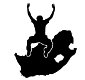
\includegraphics[width=2.5cm]{logo}} & Objectives: &
Learn how to create and edit vector and attribute data. \\
& & \\
& Keywords: & 
Editing, data capture, heads-up, table, database  \\
\hline
\end{tabular}

\subsection{Overview}\label{subsec:overview}

In the previous two topics we looked at vector data. We saw that there are
two key concepts to vector data, namely: \textbf{geometry} and
\textbf{attributes}. The
geometry of a vector feature describes its \textbf{shape} and
\textbf{position}, while the
\textbf{attributes} of a vector feature describe its \textbf{properties}
(colour, size, age etc.).

In this section we will look more closely at the process of creating and
editing vector data - both the geometry and attributes of vector features.

\subsection{How does GIS digital data get stored?}

Word processors, spreadsheets and graphics packages are all programs that let
you create and edit digital data. Each type of application saves its data
into a particular file format. For example, a graphics program will let you
save your drawing as a '.jpg' JPEG image, word processors let you save your
document as an '.odt' OpenDocument or '.doc' Word Document, and so on.

Just like these other applications, GIS Applications can store their data in
files on the computer hard disk. There are a number of different file formats
for GIS data, but the most common one is probably the 'shape file'. The name
is a little odd in that although we call it a shape file (singular), it
actually consists of at least three different files that work together to
store your digital vector data, as shown in Table \ref{tab:shapefile}. 

%% Note: xdvi does not show white text on black background but it works!
\begin{table}[ht]
\centering
\caption{The basic files that together make up a 'shapefile'.}\medskip
 \label{tab:shapefile}
 \begin{tabular}{|p{3cm}|p{13cm}|}
 \hline
 \rowcolor{black}
 \textcolor{white}{\textbf{Extension}} &
 \textcolor{white}{\textbf{Description}} \\
 \hline .shp & The geometry of vector features are stored in this file. \\
 \hline .dbf & The attributes of vector features are stored in this file. \\
 \hline .shx & This file is an index that helps the GIS Application to find
features more quickly. \\
\hline
\end{tabular}
\end{table}

When you look at the files that make up a shapefile on the computer hard
disk, you will see something like Figure \ref{fig:shapefiles}. If you want to share
vector data stored in shapefiles with another person, it is important to give
them all of the files for that layer. So in the case of the trees layer shown
in \ref{fig:shapefiles}, you would need to give the person trees.shp,
trees.shx, trees.dbf, trees.prj and trees.qml.

\begin{figure}[ht]
   \begin{center}
   \caption{The files that make up a 'trees' shapefile as seen in the
computer's file manager.}
\label{fig:shapefiles}\smallskip
   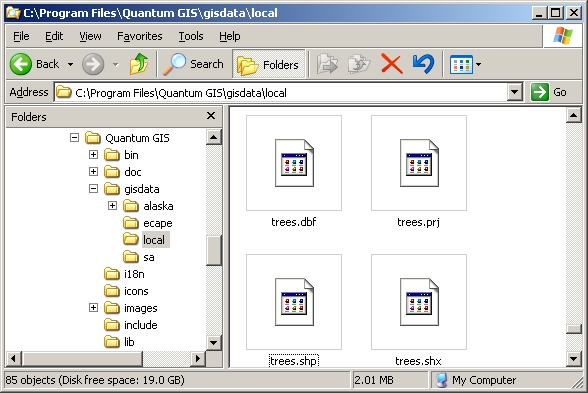
\includegraphics[clip=true, width=\textwidth]{shapefiles}
\end{center}
\end{figure}

Many GIS Applications are also able to store digital data inside a
\textbf{database}.
In general storing GIS data in a database is a good solution because the
database can store \textbf{large amounts} of data \textbf{efficiently} and
can provide data to
the GIS Application quickly. Using a database also allows many people to work
with the same vector data layers at the same time. Setting up a database to
store GIS data is more complicated than using shapefiles, so for this topic
we will focus on creating and editing shapefiles.

\subsection{Planning before you begin}

Before you can create a new vector layer (which will be stored in a
shapefile), you need know what the geometry of that layer will be (point,
polyline or polygon), and you need to know what the attributes of that layer
will be. Let's look at a few examples and it will become clearer how to go
about doing this.

\minisec{Example 1: Creating a tourism map}

Imagine that you want to create a nice tourism map for your local area. Your
vision of the final map is a 1:50 000 toposheet with markers overlaid for
sites of interest to tourists. First, let's think about the geometry. We know
that we can represent a vector layer using point, polyline or polygon
features. Which one makes the most sense for our tourism map? We could use
points if we wanted to mark specific locations such as look out points,
memorials, battle sites and so on. If we wanted to take tourists along a
route, such as a scenic oute through a mountain pass, it might make sense to
use polylines. If we have whole areas that are of tourism interest, such as a
nature reserve or a cultural village, polygons might make a good choice.

As you can see it's often not easy to know what type of geometry you will
need. One common approach to this problem is to make one layer for each
geometry type you need. So, for example, if you look at digital data provided
by the Chief Directorate : Surveys and Mapping, South Africa, they provide a
river areas (polygons) layer and a rivers polyline layer. They use the river
areas (polygons) to represent river stretches that are wide, and they use
river polylines to represent narrow stretches of river. In Figure
\ref{fig:tourism} we can see how our tourism layers might look on a map if we
used all three geometry types.

\begin{figure}[ht]
   \begin{center}
   \caption{A map with tourism layers. We have used three different geometry
types for tourism data so that we can properly represent the different kinds
of features needed for our visitors, giving them all the information they
need.}
\label{fig:tourism}\smallskip
   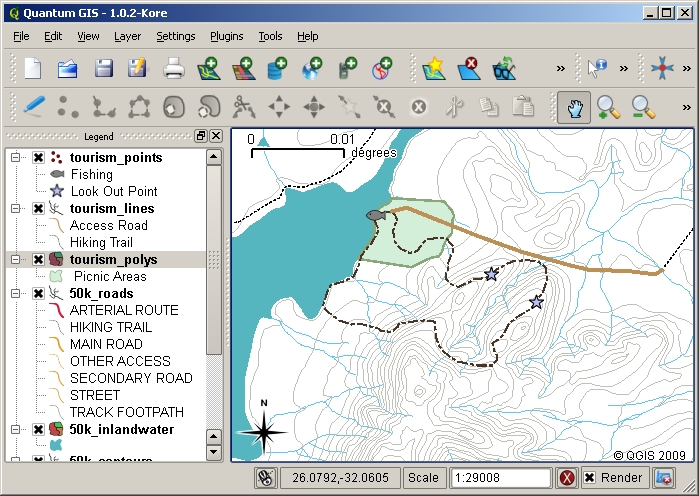
\includegraphics[clip=true, width=0.8\textwidth]{TourismMap3GeometryTypes}
\end{center}
\end{figure}

\minisec{Example 2: Creating a map of pollution levels along a river}

If you wanted to measure pollution levels along the course of a river you
would typically travel along the river in a boat or walk along its banks. At
regular intervals you would stop and take various measurements such as
Dissolved Oxygen (DO) levels, Coliform Bacteria (CB) counts, Turbidity levels
and pH. You would also need to make a map reading of your position or obtain
your position using a GPS receiver.

To store the data collected from an exercise like this in a GIS Application,
you would probably create a GIS layer with a point geometry. Using point
geometry makes sense here because each sample taken represents the conditions
at a very specific place.

For the attributes we would want a \textbf{field} for each thing that describes the
sample site. So we may end up with an attribute table that looks something
like Table \ref{tab:attrtable}.

%% Note: xdvi does not show white text on black background but it works!
\begin{table}[ht]
\centering
\caption{Drawing a table like this before you create your vector layer will
let you decide what attribute fields (columns) you will need. Note that the
geometry (positions where samples were taken) is not shown in the attribute
table - the GIS Application stores it separately!}\medskip
 \label{tab:attrtable}
 \begin{tabular}{|p{2.3cm}|p{1cm}|p{1cm}|p{1cm}|p{2.3cm}|p{2.3cm}|p{2.3cm}|}
 \hline
 \rowcolor{black}
 \textcolor{white}{\textbf{SampleNo}} &
 \textcolor{white}{\textbf{pH}} &
 \textcolor{white}{\textbf{DO}} &
 \textcolor{white}{\textbf{CB}} &
 \textcolor{white}{\textbf{Turbidity}} &
 \textcolor{white}{\textbf{Collector}} &
 \textcolor{white}{\textbf{Date}} \\
 \hline 1 & 7 & 6 & N & Low & Patience & 12/01/2009 \\
 \hline 2 & 6.8 & 5 & Y & Medium & Thabo & 12/01/2009 \\
 \hline 3 & 6.9 & 6 & Y & High & Victor & 12/01/2009 \\
\hline
\end{tabular}
\end{table}

\subsection{Creating an empty shapefile}

Once you have planned what features you want to capture into the GIS, and the
geometry type and attributes that each feature should have, you can move on
to the next step of creating an empty shapefile. 

The process usually starts with choosing the 'new vector layer' option in
your GIS Application and then selecting a \textbf{geometry type} (see Figure
\ref{fig:newshape}). As we covered in an earlier topic, this means choosing
either point, polyline or polygon for the geometry. 

\begin{figure}[ht]
   \begin{center}
   \caption{Creating a new vector layer is as simple as filling in a few
details in a form. First you choose the geometry type, and then you add the
attribute fields.}
\label{fig:newshape}\smallskip
   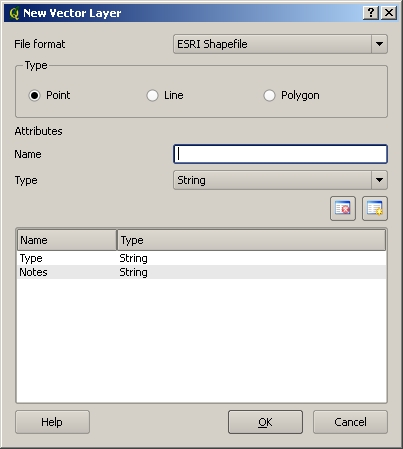
\includegraphics[clip=true, width=0.6\textwidth]{NewVectorLayer}
\end{center}
\end{figure}

Next you will add fields to the attribute table. Normally we give field names
that are short, have no spaces and indicate what type of information is being
stored in that field. Example field names may be 'pH', 'RoofColour',
'RoadType' and so on. As well as choosing a name for each field, you need to
indicate how the information should be stored in that field - i.e. is it a
number, a word or a sentence, or a date? 

Computer programs usually call information that is made up of words or
sentences '\textbf{strings}', so if you need to store something like a street name or
the name of a river, you should use string for the field type.

The shapefile format allows you to store the numeric field information as
either a whole number (\textbf{integer}) or a decimal number
(\textbf{floating point}) - so you
need to think before hand whether the numeric data you are going to capture
will have decimal places or not.

\begin{figure}[ht]
   \begin{center}
   \caption{After defining our new layer's geometry and attributes, we need
to save it to disk. It is important to give a short but meaningful name to
your shapefile.}
\label{fig:saveas}\smallskip
   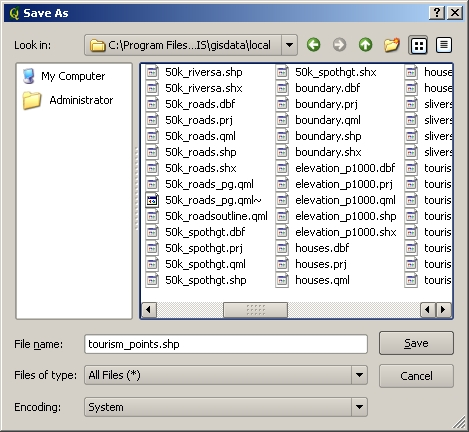
\includegraphics[clip=true, width=0.6\textwidth]{SaveAs}
\end{center}
\end{figure}

The final step (as shown in Figure \ref{fig:saveas}) for creating a shapefile
is
to give it a name and a place on the computer hard disk where it should be
created. Once again it is a good idea to give the shapefile a short and
meaningful name. Good examples are 'rivers', 'watersamples' and so on.

Let's recap the process again quickly. To create a shapefile you first say
what kind of geometry it will hold, then you create one or more fields for
the attribute table, and then you save the shapefile to the hard disk using
an easy to recognise name. Easy as 1-2-3!

\subsection{Adding data to your shapefile}

So far we have only created an empty shapefile. Now we need to \textbf{enable
editing}
in the shapefile using the 'enable editing' menu option or tool bar icon in
the GIS Application. Shapefiles are not enabled for editing by default to
prevent accidentally changing or deleting the data they contain. Next we need
to start adding data. There are two steps we need to complete for each
\textbf{record} we add to the shapefile:

\begin{enumerate}
\item Capturing geometry
\item Entering attributes 
\end{enumerate}

The process of capturing geometry is different for points, polylines and
polygons. 

To \textbf{capture a point}, you first use the map pan and zoom tools to get to the
correct geographical area that you are going to be recording data for. Next
you will need to enable the point capture tool. Having done that, the next
place you click with the \textbf{left mouse button} in the map view, is where you want
your new point \textbf{geometry} to appear. After you click on the map, a window will
appear and you can enter all of the \textbf{attribute data} for that point (see
Figure \ref{fig:enterattr}). If you are unsure of the data for a given field you
can usually leave it blank, but be aware that if you leave a lot of fields
blank it will be hard to make a useful map from your data!

\begin{figure}[ht]
   \begin{center}
   \caption{After you have captured the point geometry, you will be asked to
describe its attributes. The attribute form is based on the fields you
specified when you created the vector layer.}
\label{fig:enterattr}\smallskip
   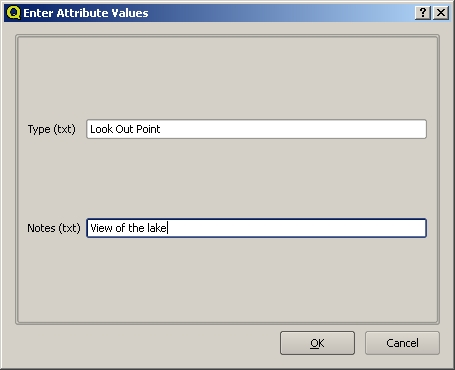
\includegraphics[clip=true, width=0.5\textwidth]{EnterAttributeValues}
\end{center}
\end{figure}

To \textbf{capture a polyline} the process is similar to that of a point, in that you
need to first use the pan and zoom tools to move the map in the map view to
the correct geographical area. You should be zoomed in enough so that your
new vector polyline feature will have an appropriate scale (see Topic 2:
Working with Vector Data for more details on scale issues). When you are
ready, you can click the polyline capture icon in the tool bar and then start
drawing your line by clicking on the map. After you make your first click,
you will notice that the line stretches like an elastic band to follow the
mouse cursor around as you move it. Each time you click with the \textbf{left
mouse button}, a new vertex will be added to the map. This process is shown in
Figure \ref{fig:linecapture}. 

\begin{figure}[ht]
   \begin{center}
   \caption{Capturing lines for a tourism map. When editing a line layer, the
vertices are shown with circular markers which you can move about with the
mouse to adjust the line's geometry. When adding a new line (shown in red),
each click of the mouse will add a new vertex.}
\label{fig:linecapture}\smallskip
   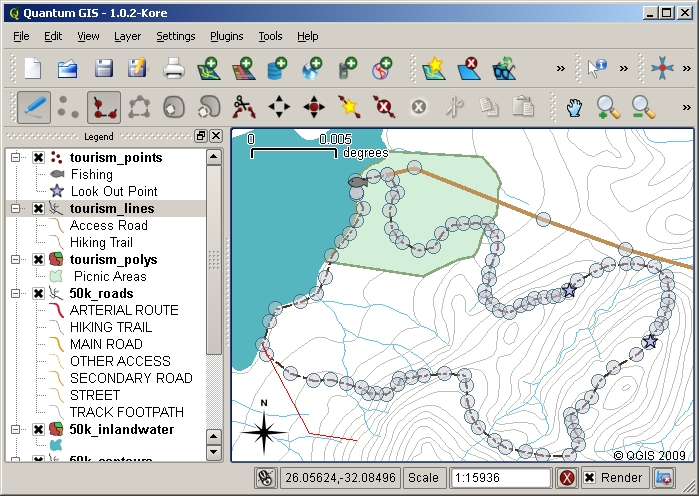
\includegraphics[clip=true, width=\textwidth]{LineCapture}
\end{center}
\end{figure}

When you have finished defining your line, use the \textbf{right mouse
button} to tell
the GIS Application that you have completed your edits. As with the procedure
for capturing a point feature, you will then be asked to enter in the
attribute data for your new polyline feature.

The process for \textbf{capturing a polygon} is almost the same as capturing a
polyline except that you need to use the polygon capture tool in the tool
bar. Also, you will notice that when you draw your geometry on the screen,
the GIS Application always creates an enclosed area.

To add a new feature after you have created your first one, you can simply
click again on the map with the point, polyline or polygon capture tool
active and start to draw your next feature.

When you have no more features to add, always be sure to click the 'allow
editing' icon to toggle it off. The GIS Application will then save your newly
created layer to the hard disk.

\subsection{Heads-up digitising}

As you have probably discovered by now if you followed the steps above, it is
pretty hard to draw the features so that they are \textbf{spatially correct} if you do
not have other features that you can use as a point of reference. One common
solution to this problem is to use a raster layer (such as an aerial
photograph or a satellite image) as a backdrop layer. You can then use this
layer as a reference map, or even trace the features off the raster layer
into your vector layer if they are visible. This process is known as
'heads-up digitising' and is shown in Figure \ref{fig:headsupdigi}.

\begin{figure}[ht]
   \begin{center}
   \caption{Heads-up digitising using a satellite image as a backdrop. The
image is used as a reference for capturing polyline features by tracing over
them.}
\label{fig:headsupdigi}\smallskip
   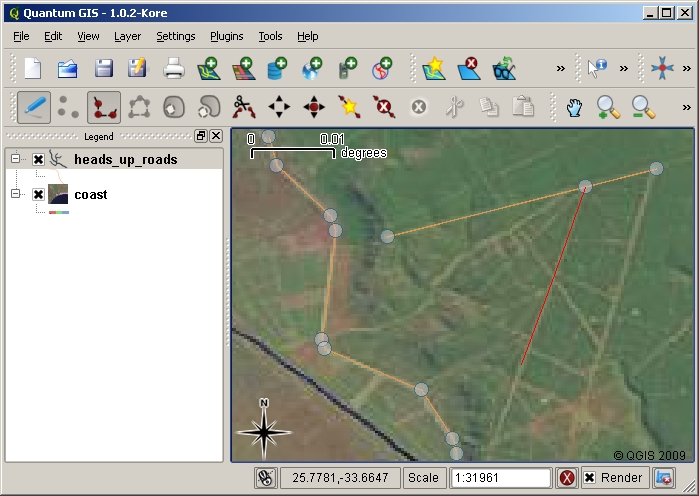
\includegraphics[clip=true, width=\textwidth]{HeadsUpDigitising}
\end{center}
\end{figure}

\subsection{Digitising using a digitising table}

Another method of capturing vector data is to use a digitising table. This
approach is less commonly used except by GIS professionals, and it requires
expensive equipment. The process of using a digitising table, is to place a
paper map on the table. The paper map is held securely in place using clips.
Then a special device called a 'puck' is used to trace features from the map.
Tiny cross-hairs in the puck are used to ensure that lines and points are
drawn accurately. The puck is connected to a computer and each feature that
is captured using the puck gets stored in the computer's memory. You can see
what a digitising puck looks like in Figure \ref{fig:digitable}.

\begin{figure}[htpb]
   \begin{center}
   \caption{A digitising table and puck are used by GIS professionals when
they want to digitise features from existing maps.}
\label{fig:digitable}\smallskip
   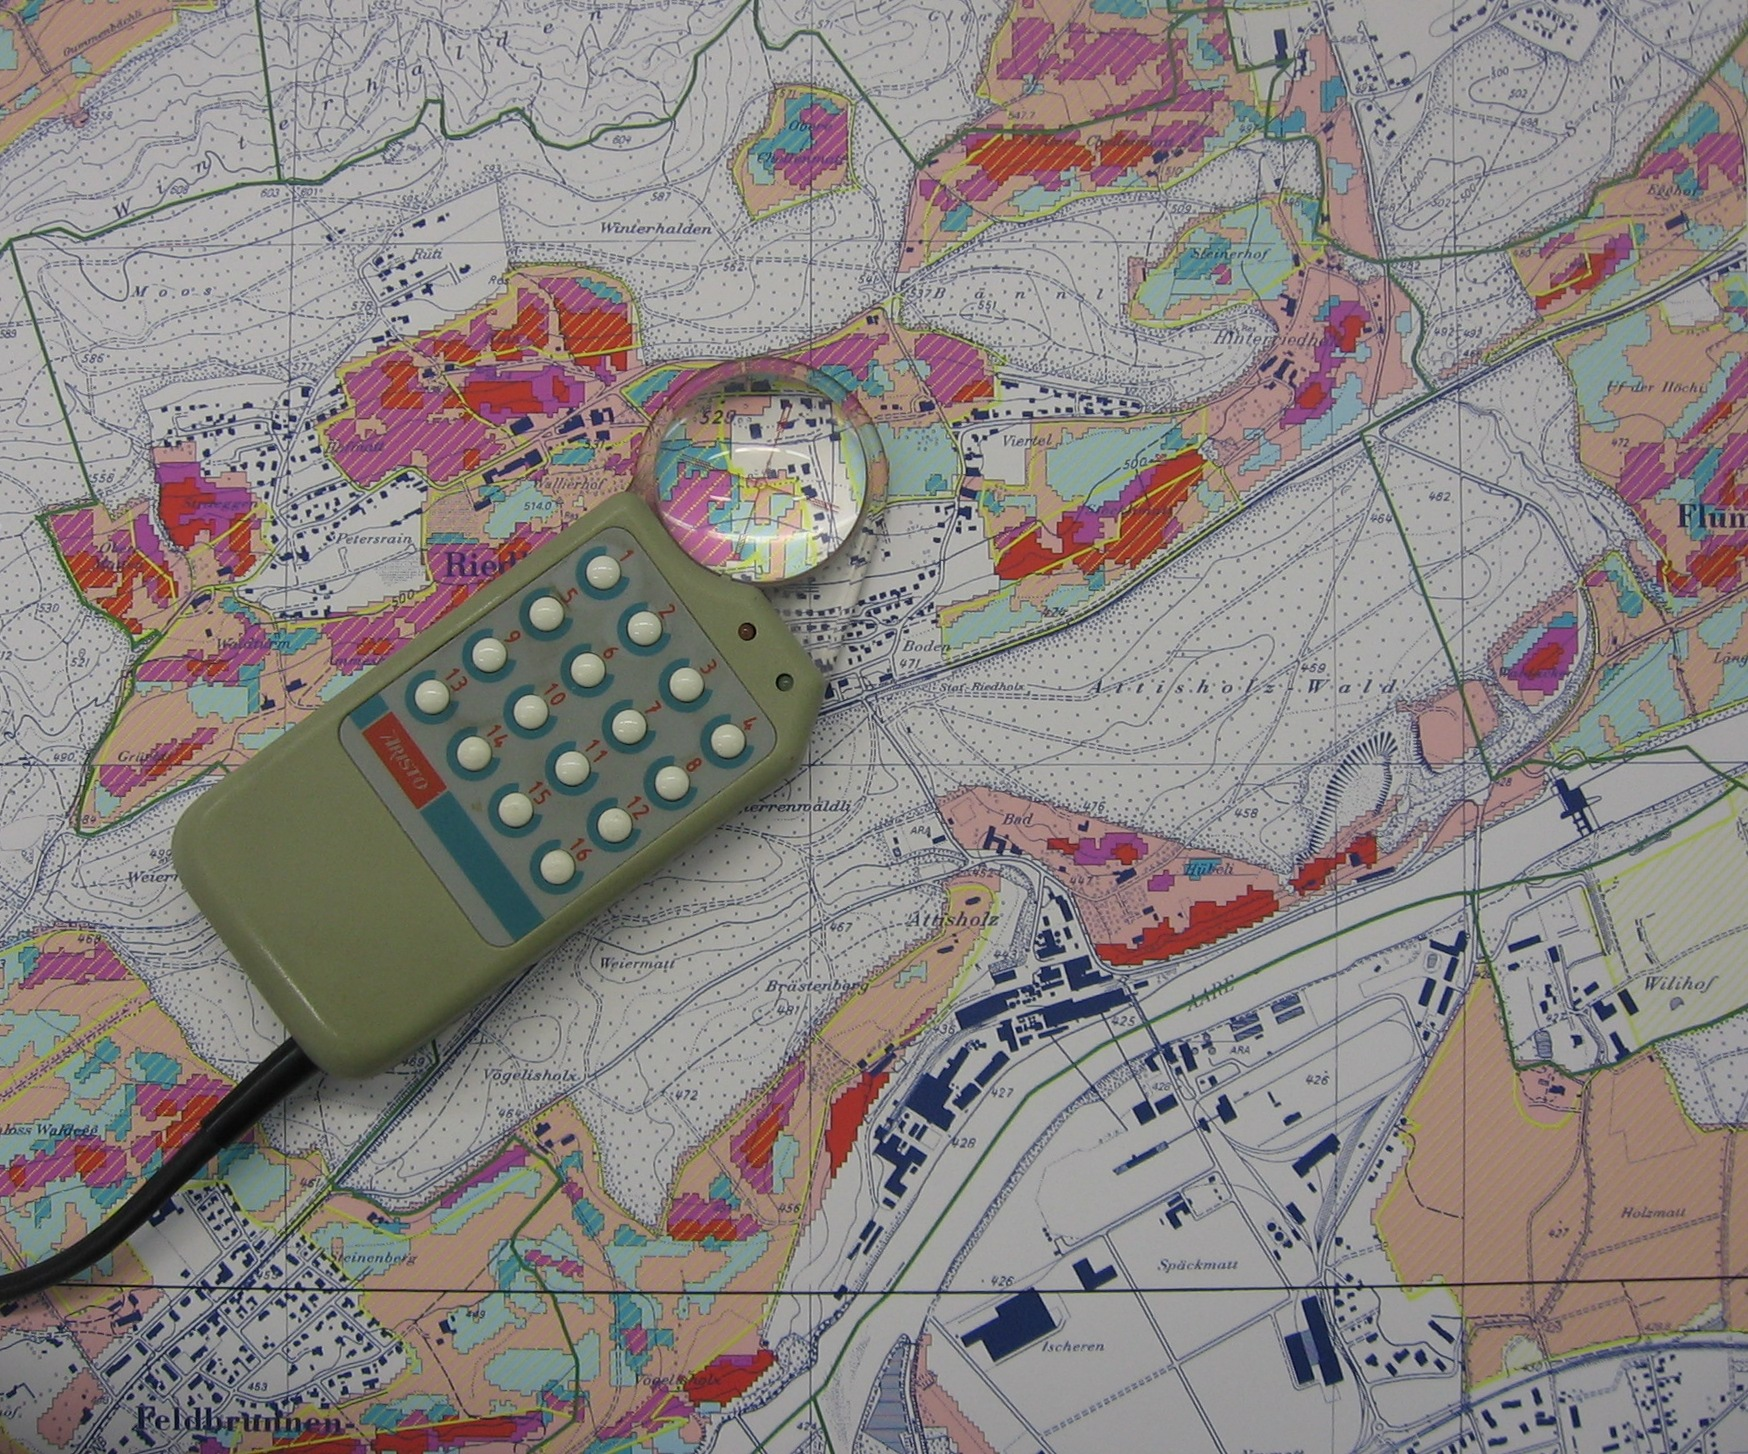
\includegraphics[clip=true, width=\textwidth]{digitising_table}
\end{center}
\end{figure}

\minisec{After your features are digitised}

Once your features are digitised, you can use the techniques you learned in
the previous Topic to set the symbology for your layer. Choosing an
appropriate symbology will allow you to better understand the data you have
captured when you look at the map.

\subsection{Common problems / things to be aware of}

If you are digitising using a backdrop raster layer such as an aerial
photograph or satellite image, it is very important that the raster layer is
properly georeferenced. A layer that is georeferenced properly displays in
the correct position in the map view based on the GIS Application's internal
model of the earth. We can see the effect of a poorly georeferenced image in
Figure \ref{fig:refgoodbad}.

\begin{figure}[ht]
   \begin{center}
   \caption{The importance of using properly georeferenced raster images for
heads-up digitising.  On the left we can see the image is properly
georegistered and the road features (in orange) overlap perfectly. If the
image is poorly georeferenced (as shown on the right) the features will not
be well aligned. Worse still, if the image on the right is used as a
reference when capturing new features, the newly captured data will be
inaccurate!}
\label{fig:refgoodbad}\smallskip
   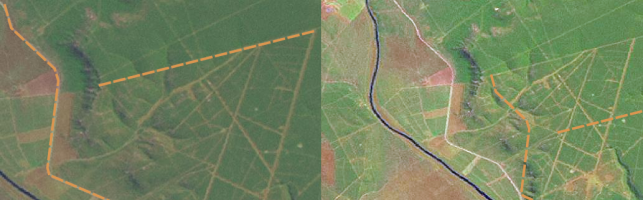
\includegraphics[clip=true, width=\textwidth]{GeoreferencingGoodVsBad}
\end{center}
\end{figure}

Also remember that it is important that you are zoomed in to an appropriate
scale so that the vector features you create are useful. As we saw in the
previous topic on vector geometry, it is a bad idea to digitise your data
when you are zoomed out to a scale of 1:1000 000 if you intend to use the
data you capture at a scale of 1:50 000 later.

\subsection{What have we learned?}

Let's wrap up what we covered in this worksheet:

\begin{itemize}
\item \textbf{Digitising} is the process of capturing knowledge of a
feature's \textbf{geometry} and \textbf{attributes} into a \textbf{digital
format} stored on the computer's disk.
\item GIS Data can be stored in a \textbf{database} or as \textbf{files}.
\item One commonly used file format is the \textbf{shapefile} which is
actually a group of three or more files (.shp, .dbf and .shx).
\item Before you create a new vector layer you need to plan both what
\textbf{geometry} type and \textbf{attribute} fields it will contain.
\item Geometry can be point, polyline or polygon.
\item Attributes can be \textbf{integers} (whole numbers), \textbf{floating
points} (decimal numbers), \textbf{strings} (words) or \textbf{dates}.
\item The digitising process consists of \textbf{drawing} the geometry in the
map view and then entering its attributes. This is repeated for each feature.
\item \textbf{Heads-up digitising} is often used to provide orientation
during digitising by using a raster image in the background.
\item Professional GIS users sometimes use a \textbf{digitising table} to
capture information from paper maps.
\end{itemize}

\subsection{Now you try!}

Here are some ideas for you to try with your learners:

\begin{itemize}
\item Draw up a list of features in and around your school that you think would be
interesting to capture. For example: the school boundary, the position of
fire assembly points, the layout of each class room, and so on. Try to use a
mix of different geometry types. Now split your learners into groups and
assign each group a few features to capture. Have them symbolise their layers
so that they are more meaningful to look at. Combine the layers from all the
groups to create a nice map of your school and its surroundings!
\item Find a local river and take water samples along its length. Make a careful
note of the position of each sample using a GPS or by marking it on a
toposheet. For each sample take measurements such as pH, dissolved oxygen
etc. Capture the data using the GIS application and make maps that show the
samples with a suitable symbology. Could you identify any areas of concern?
Was the GIS Application able to help you to identify these areas?
\end{itemize}

\subsection{Something to think about}

If you don't have a computer available, you can follow the same process by
using transparency sheets and a notebook. Use an aerial photo, orthosheet or
satellite image printout as your background layer. Draw columns down the page
in your notebook and write in the column headings for each attribute field
you want to store information about. Now trace the geometry of features onto
the transparency sheet, writing a number next to each feature so that it can
be identified. Now write the same number in the first column in your table in
your notebook, and then fill in all the additional information you want to
record.

\subsection{Further reading}

\textbf{Website}:

\url{http://www.k12science.org/curriculum/waterproj/S00project/miami2000/miamiriverfinal.html} - A school project to assess water quality in their local river.

The QGIS User Guide also has more detailed information on digitising vector
data in QGIS.

\subsection{What's next?}

In the section that follows we will take a closer look at raster data to
learn all about how image data can be used in a GIS.






